\documentclass{standalone}
\usepackage{tikz}
\usetikzlibrary{patterns, positioning}
\usepackage[sfdefault]{ClearSans} %% option 'sfdefault' activates Clear Sans as the default text font
\usepackage[T1]{fontenc}

\begin{document}
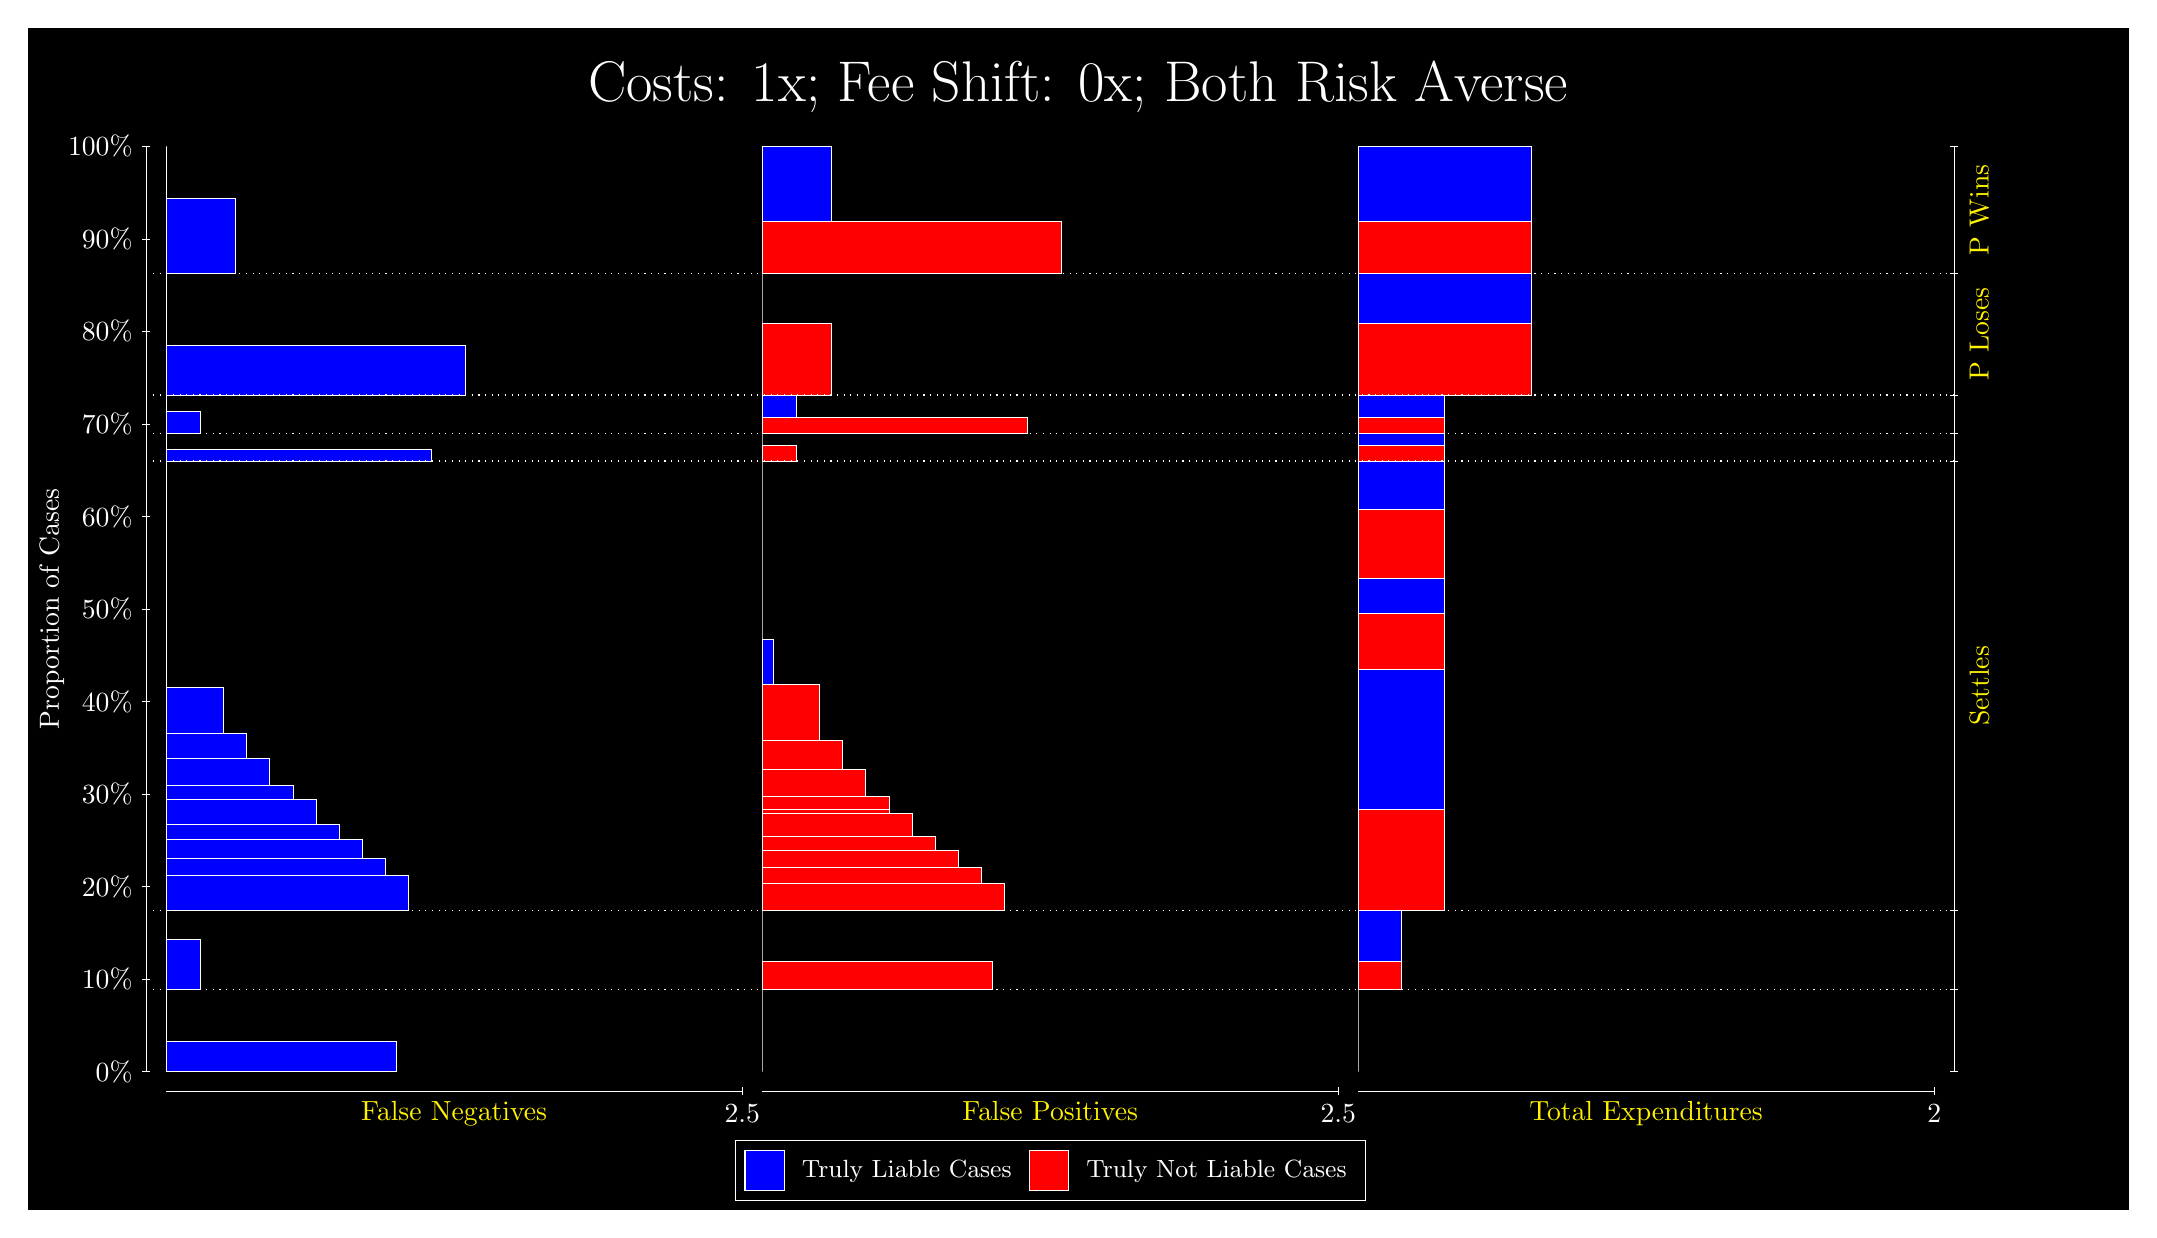
\begin{tikzpicture}
\draw[fill=black] (0,0) rectangle (26.667,15);
\draw[text=white] (0,13.5) rectangle (26.667,15) node[midway] {\huge Costs: 1x; Fee Shift: 0x; Both Risk Averse};
\draw[white, very thin] (1.5,1.75) -- (1.5,13.5);
\node[rotate=90, text=white, anchor=center] at (0.3, 7.625) {Proportion of Cases};
\draw[white, very thin] (1.45,1.75) -- (1.55,1.75);
\node[text=white, anchor=east] at (1.45, 1.75) {0\%};
\draw[white, very thin] (1.45,2.925) -- (1.55,2.925);
\node[text=white, anchor=east] at (1.45, 2.925) {10\%};
\draw[white, very thin] (1.45,4.1) -- (1.55,4.1);
\node[text=white, anchor=east] at (1.45, 4.1) {20\%};
\draw[white, very thin] (1.45,5.275) -- (1.55,5.275);
\node[text=white, anchor=east] at (1.45, 5.275) {30\%};
\draw[white, very thin] (1.45,6.45) -- (1.55,6.45);
\node[text=white, anchor=east] at (1.45, 6.45) {40\%};
\draw[white, very thin] (1.45,7.625) -- (1.55,7.625);
\node[text=white, anchor=east] at (1.45, 7.625) {50\%};
\draw[white, very thin] (1.45,8.8) -- (1.55,8.8);
\node[text=white, anchor=east] at (1.45, 8.8) {60\%};
\draw[white, very thin] (1.45,9.975) -- (1.55,9.975);
\node[text=white, anchor=east] at (1.45, 9.975) {70\%};
\draw[white, very thin] (1.45,11.15) -- (1.55,11.15);
\node[text=white, anchor=east] at (1.45, 11.15) {80\%};
\draw[white, very thin] (1.45,12.325) -- (1.55,12.325);
\node[text=white, anchor=east] at (1.45, 12.325) {90\%};
\draw[white, very thin] (1.45,13.5) -- (1.55,13.5);
\node[text=white, anchor=east] at (1.45, 13.5) {100\%};

\draw[white, very thin] (24.457,1.75) -- (24.457,13.5);
\draw[white, very thin] (24.407,1.75) -- (24.507,1.75);
\node[anchor=west] at (24.407, 1.75) {};
\draw[white, very thin] (24.407,2.7974) -- (24.507,2.7974);
\node[anchor=west] at (24.407, 2.7974) {};
\draw[white, very thin] (24.407,3.7917) -- (24.507,3.7917);
\node[anchor=west] at (24.407, 3.7917) {};
\draw[white, very thin] (24.407,9.5032) -- (24.507,9.5032);
\node[anchor=west] at (24.407, 9.5032) {};
\draw[white, very thin] (24.407,9.8572) -- (24.507,9.8572);
\node[anchor=west] at (24.407, 9.8572) {};
\draw[white, very thin] (24.407,10.342) -- (24.507,10.342);
\node[anchor=west] at (24.407, 10.342) {};
\draw[white, very thin] (24.407,11.886) -- (24.507,11.886);
\node[anchor=west] at (24.407, 11.886) {};
\draw[white, very thin] (24.407,13.5) -- (24.507,13.5);
\node[anchor=west] at (24.407, 13.5) {};

\draw[white, very thin, fill=blue] (1.75,1.75) rectangle (4.6775,2.1312);
\draw[white, very thin, fill=red] (1.75,2.1312) rectangle (1.75,2.7974);
\draw[white, very thin, fill=blue] (1.75,2.7974) rectangle (2.1891,3.4353);
\draw[white, very thin, fill=red] (1.75,3.4353) rectangle (1.75,3.7917);
\draw[white, very thin, fill=blue] (1.75,3.7917) rectangle (4.8239,4.2363);
\draw[white, very thin, fill=blue] (1.75,4.2363) rectangle (4.5312,4.4612);
\draw[white, very thin, fill=blue] (1.75,4.4612) rectangle (4.2384,4.6944);
\draw[white, very thin, fill=blue] (1.75,4.6944) rectangle (3.9457,4.8953);
\draw[white, very thin, fill=blue] (1.75,4.8953) rectangle (3.6529,5.2026);
\draw[white, very thin, fill=blue] (1.75,5.2026) rectangle (3.3602,5.3882);
\draw[white, very thin, fill=blue] (1.75,5.3882) rectangle (3.0674,5.7247);
\draw[white, very thin, fill=blue] (1.75,5.7247) rectangle (2.7746,6.0489);
\draw[white, very thin, fill=blue] (1.75,6.0489) rectangle (2.4819,6.6246);
\draw[white, very thin, fill=red] (1.75,6.6246) rectangle (1.75,9.5032);
\draw[white, very thin, fill=blue] (1.75,9.5032) rectangle (5.1167,9.6508);
\draw[white, very thin, fill=red] (1.75,9.6508) rectangle (1.75,9.8572);
\draw[white, very thin, fill=blue] (1.75,9.8572) rectangle (2.1891,10.141);
\draw[white, very thin, fill=red] (1.75,10.141) rectangle (1.75,10.342);
\draw[white, very thin, fill=blue] (1.75,10.342) rectangle (5.5558,10.979);
\draw[white, very thin, fill=red] (1.75,10.979) rectangle (1.75,11.886);
\draw[white, very thin, fill=blue] (1.75,11.886) rectangle (2.6283,12.841);
\draw[white, very thin, fill=red] (1.75,12.841) rectangle (1.75,13.5);
\draw[white, very thin, fill=red] (9.3189,1.75) rectangle (9.3189,2.4162);
\draw[white, very thin, fill=blue] (9.3189,2.4162) rectangle (9.3189,2.7974);
\draw[white, very thin, fill=red] (9.3189,2.7974) rectangle (12.246,3.1538);
\draw[white, very thin, fill=blue] (9.3189,3.1538) rectangle (9.3189,3.7917);
\draw[white, very thin, fill=red] (9.3189,3.7917) rectangle (12.393,4.145);
\draw[white, very thin, fill=red] (9.3189,4.145) rectangle (12.1,4.3433);
\draw[white, very thin, fill=red] (9.3189,4.3433) rectangle (11.807,4.563);
\draw[white, very thin, fill=red] (9.3189,4.563) rectangle (11.515,4.7327);
\draw[white, very thin, fill=red] (9.3189,4.7327) rectangle (11.222,5.035);
\draw[white, very thin, fill=red] (9.3189,5.035) rectangle (10.929,5.0851);
\draw[white, very thin, fill=red] (9.3189,5.0851) rectangle (10.929,5.2484);
\draw[white, very thin, fill=red] (9.3189,5.2484) rectangle (10.636,5.5941);
\draw[white, very thin, fill=red] (9.3189,5.5941) rectangle (10.344,5.9583);
\draw[white, very thin, fill=red] (9.3189,5.9583) rectangle (10.051,6.6703);
\draw[white, very thin, fill=blue] (9.3189,6.6703) rectangle (9.4652,7.2459);
\draw[white, very thin, fill=blue] (9.3189,7.2459) rectangle (9.3189,9.5032);
\draw[white, very thin, fill=red] (9.3189,9.5032) rectangle (9.758,9.7096);
\draw[white, very thin, fill=blue] (9.3189,9.7096) rectangle (9.3189,9.8572);
\draw[white, very thin, fill=red] (9.3189,9.8572) rectangle (12.686,10.059);
\draw[white, very thin, fill=blue] (9.3189,10.059) rectangle (9.758,10.342);
\draw[white, very thin, fill=red] (9.3189,10.342) rectangle (10.197,11.249);
\draw[white, very thin, fill=blue] (9.3189,11.249) rectangle (9.3189,11.886);
\draw[white, very thin, fill=red] (9.3189,11.886) rectangle (13.125,12.545);
\draw[white, very thin, fill=blue] (9.3189,12.545) rectangle (10.197,13.5);
\draw[white, very thin, fill=red] (16.888,1.75) rectangle (16.888,2.4162);
\draw[white, very thin, fill=blue] (16.888,2.4162) rectangle (16.888,2.7974);
\draw[white, very thin, fill=red] (16.888,2.7974) rectangle (17.437,3.1538);
\draw[white, very thin, fill=blue] (16.888,3.1538) rectangle (17.437,3.7917);
\draw[white, very thin, fill=red] (16.888,3.7917) rectangle (17.986,5.0851);
\draw[white, very thin, fill=blue] (16.888,5.0851) rectangle (17.986,6.8601);
\draw[white, very thin, fill=red] (16.888,6.8601) rectangle (17.986,7.572);
\draw[white, very thin, fill=blue] (16.888,7.572) rectangle (17.986,8.0167);
\draw[white, very thin, fill=red] (16.888,8.0167) rectangle (17.986,8.8899);
\draw[white, very thin, fill=blue] (16.888,8.8899) rectangle (17.986,9.5032);
\draw[white, very thin, fill=red] (16.888,9.5032) rectangle (17.986,9.7096);
\draw[white, very thin, fill=blue] (16.888,9.7096) rectangle (17.986,9.8572);
\draw[white, very thin, fill=red] (16.888,9.8572) rectangle (17.986,10.059);
\draw[white, very thin, fill=blue] (16.888,10.059) rectangle (17.986,10.342);
\draw[white, very thin, fill=red] (16.888,10.342) rectangle (19.083,11.249);
\draw[white, very thin, fill=blue] (16.888,11.249) rectangle (19.083,11.886);
\draw[white, very thin, fill=red] (16.888,11.886) rectangle (19.083,12.545);
\draw[white, very thin, fill=blue] (16.888,12.545) rectangle (19.083,13.5);
\draw[white, dotted] (1.5,2.7974) -- (24.457,2.7974);
\draw[white, dotted] (1.5,3.7917) -- (24.457,3.7917);
\draw[white, dotted] (1.5,9.5032) -- (24.457,9.5032);
\draw[white, dotted] (1.5,9.8572) -- (24.457,9.8572);
\draw[white, dotted] (1.5,10.342) -- (24.457,10.342);
\draw[white, dotted] (1.5,11.886) -- (24.457,11.886);
\draw[white, very thin] (1.75,1.5) -- (9.0689,1.5);
\node[text=yellow, anchor=north] at (5.4094, 1.5) {False Negatives};
\draw[white, very thin] (9.0689,1.45) -- (9.0689,1.55);
\node[text=white, anchor=north] at (9.0689, 1.45) {2.5};

\draw[white, very thin] (9.3189,1.5) -- (16.638,1.5);
\node[text=yellow, anchor=north] at (12.978, 1.5) {False Positives};
\draw[white, very thin] (16.638,1.45) -- (16.638,1.55);
\node[text=white, anchor=north] at (16.638, 1.45) {2.5};

\draw[white, very thin] (16.888,1.5) -- (24.207,1.5);
\node[text=yellow, anchor=north] at (20.547, 1.5) {Total Expenditures};
\draw[white, very thin] (24.207,1.45) -- (24.207,1.55);
\node[text=white, anchor=north] at (24.207, 1.45) {2};



\node[text=yellow, centered, rotate=90] at (24.777, 6.6474) {Settles};


\node[text=yellow, centered, rotate=90] at (24.777, 11.114) {P Loses};
\node[text=yellow, centered, rotate=90] at (24.777, 12.693) {P Wins};

\draw (12.978300999999998,1.5) node[draw=none] (baseCoordinate) {};
\begin{scope}[align=center]
        \matrix[scale=0.5, draw=white, below=0.5cm of baseCoordinate, nodes={draw}, column sep=0.1cm]{
            \node[rectangle, draw, minimum width=0.5cm, minimum height=0.5cm, fill=blue] {}; &
            \node[draw=none, font=\small, text=white] (B) {Truly Liable Cases}; &
            \node[rectangle, draw, minimum width=0.5cm, minimum height=0.5cm, fill=red] {}; &
            \node[draw=none, font=\small, text=white] (B) {Truly Not Liable Cases}; \\
            };
\end{scope}

\end{tikzpicture}
\end{document}